\begin{figure}[t]
\centering
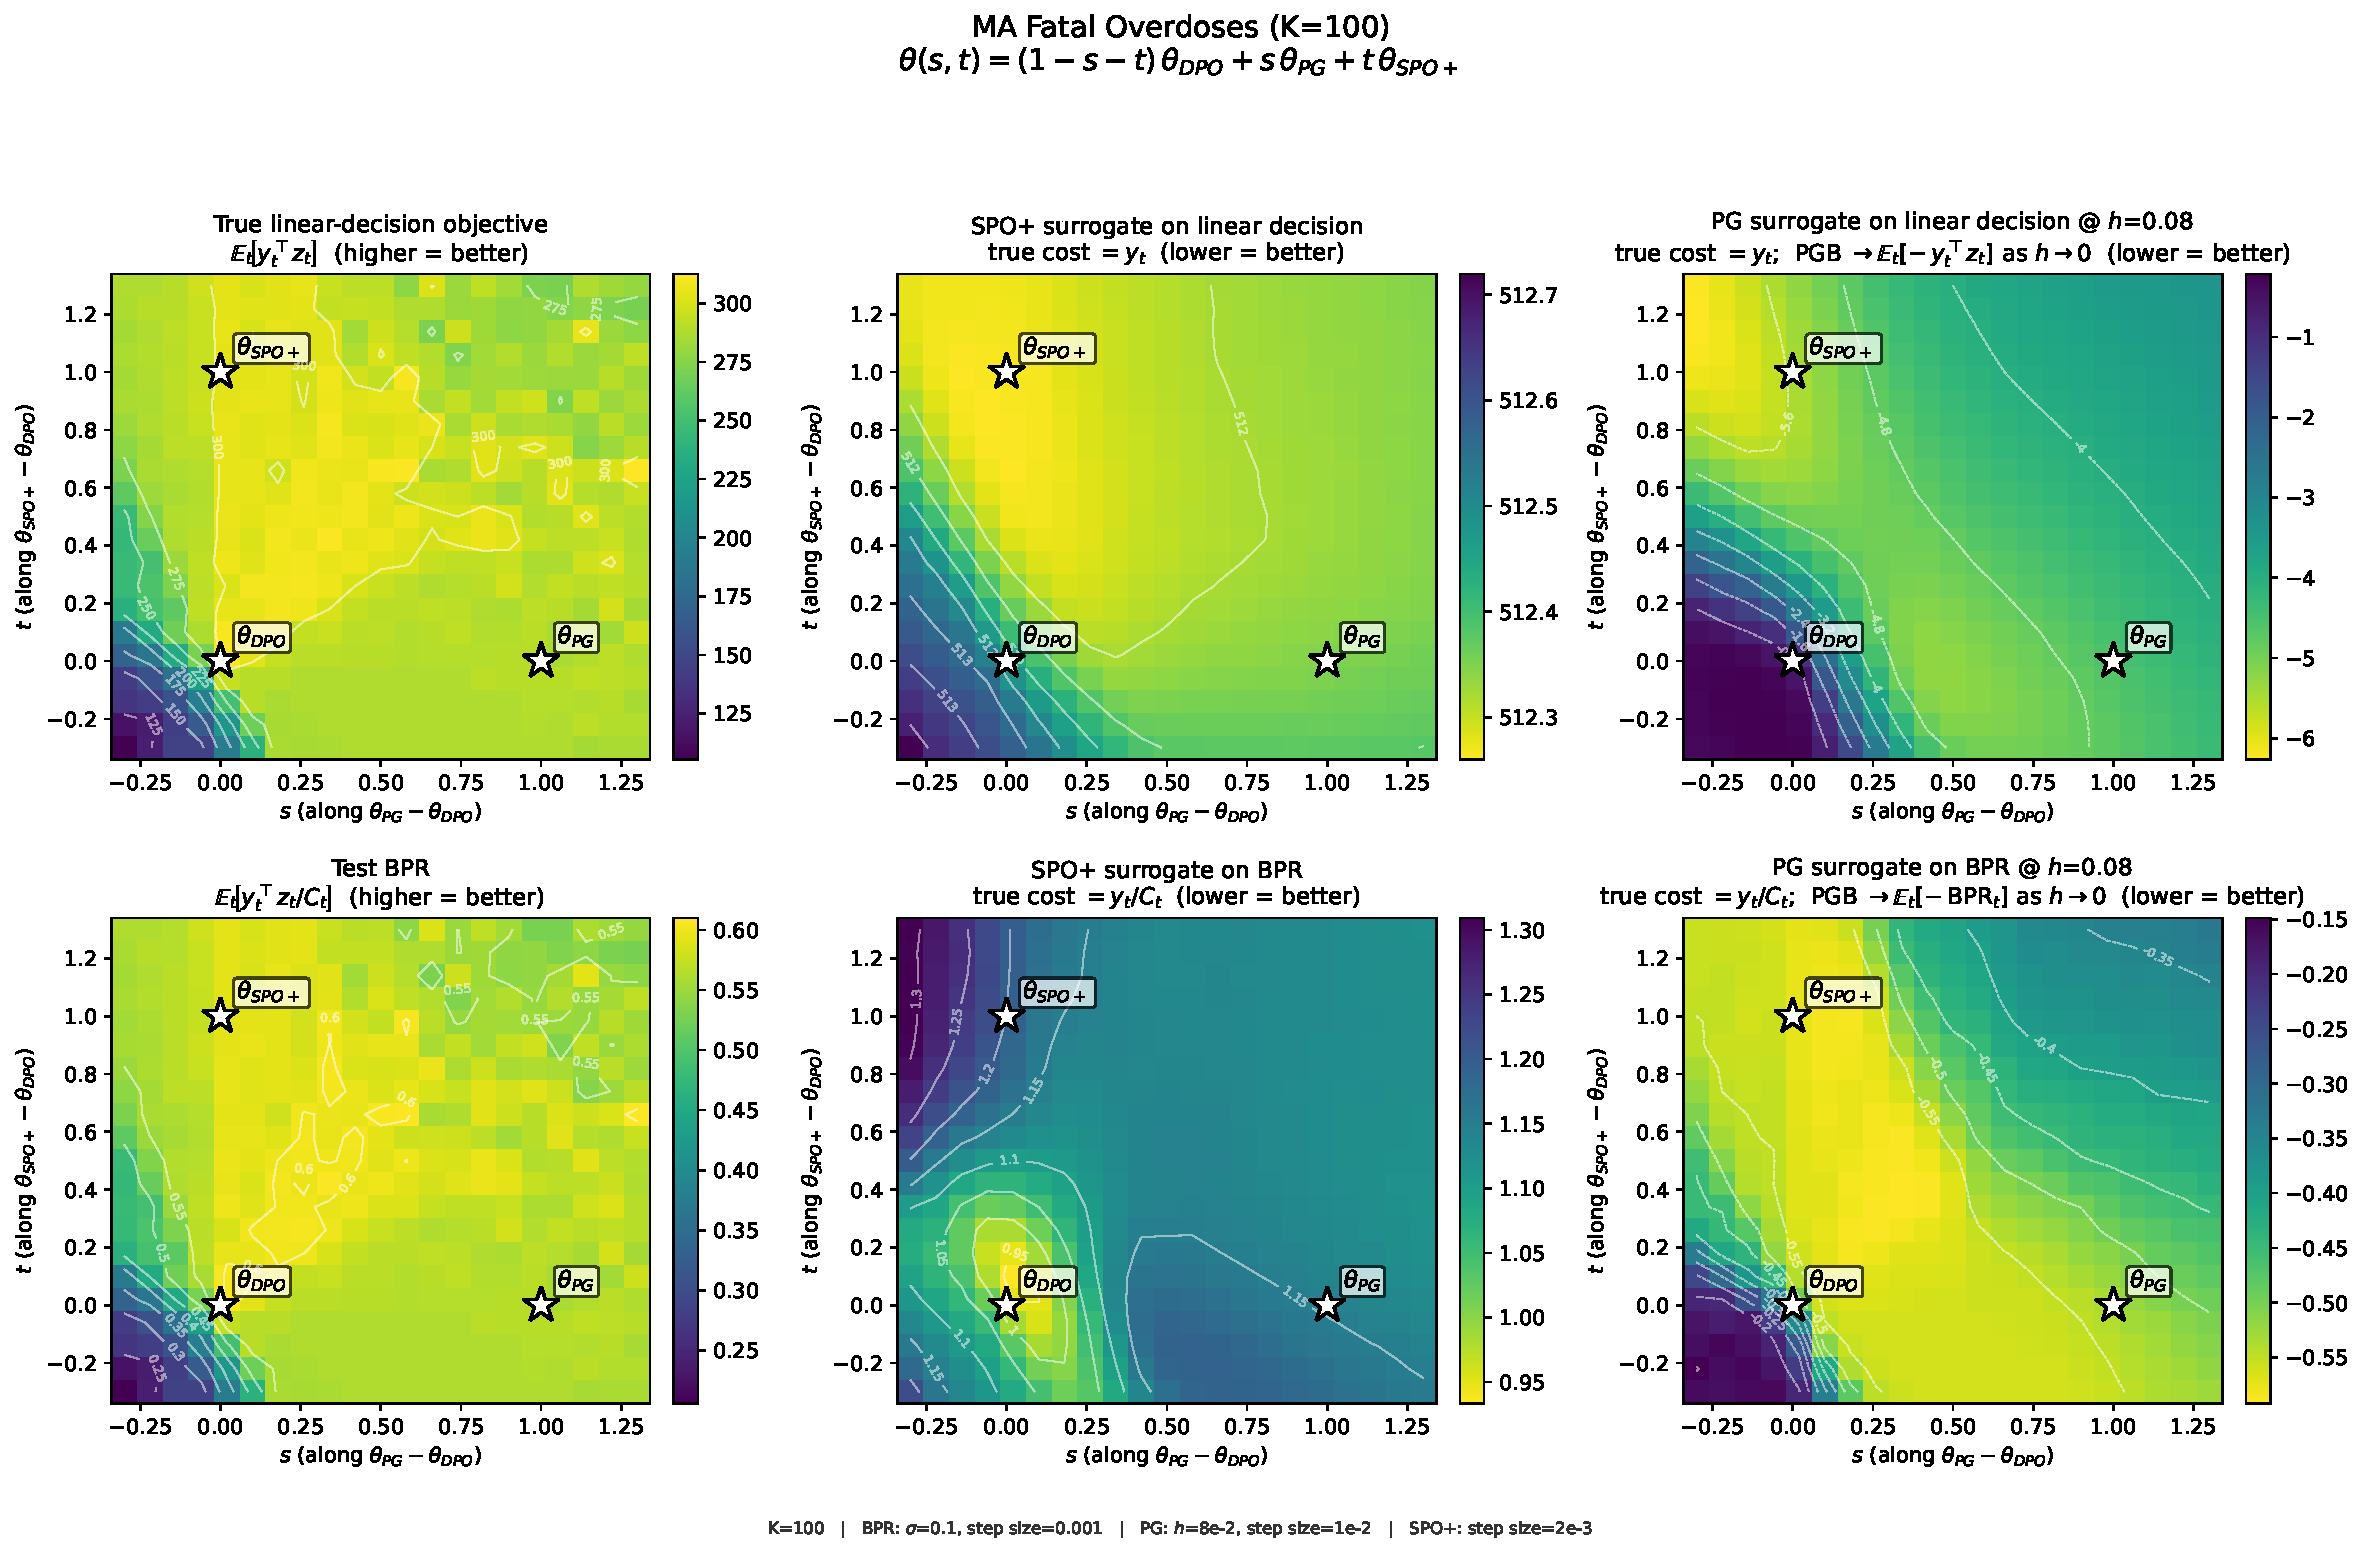
\includegraphics[width=\linewidth]{figures/hyperplane_landscape_MA.pdf}

\vspace{0.4em}
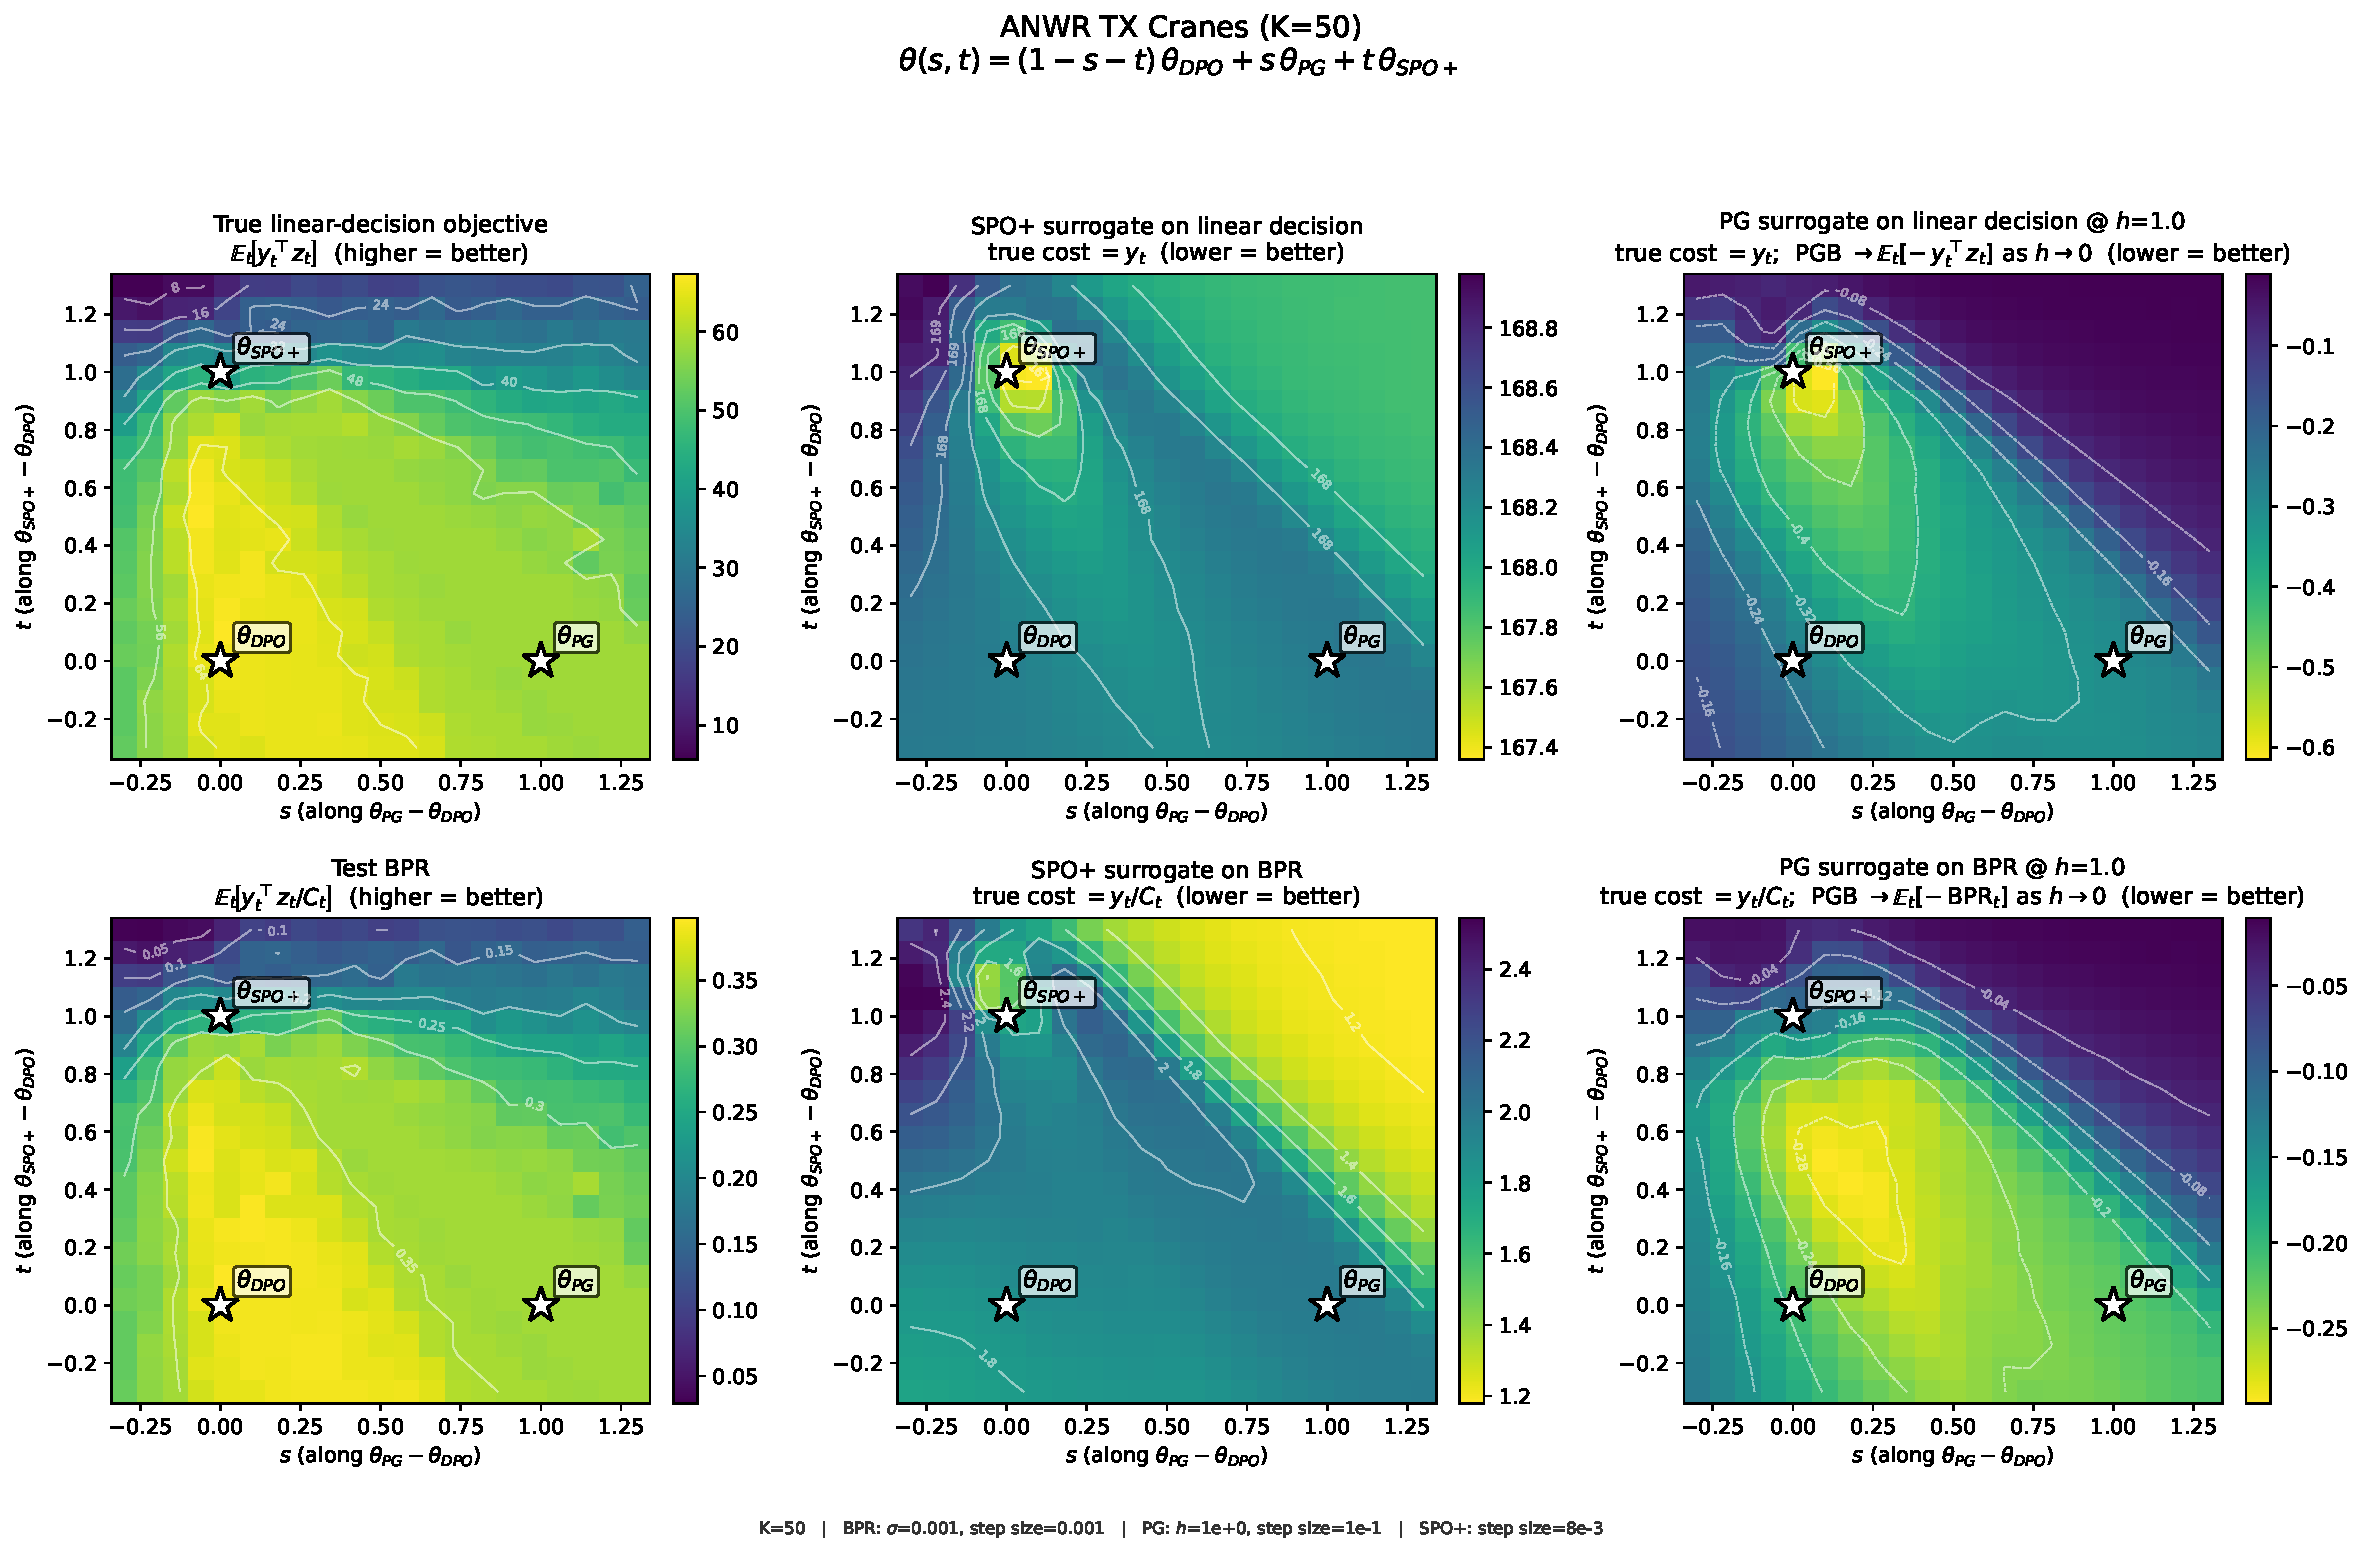
\includegraphics[width=\linewidth]{figures/hyperplane_landscape_asurv.pdf}

\vspace{-0.3em}
\setlength{\abovecaptionskip}{2pt}
\setlength{\belowcaptionskip}{0pt}
\caption[Top-K site selection: loss landscapes on the affine hyperplane for the Massachusetts opioid and aerial-survey tasks.]{\textbf{Top-K site selection on Massachusetts opioid (top) and Aransas aerial survey (bottom).} Same construction as Fig.~\ref{fig:topK_interpolation_main}: heldout-test BPR, NLL, SPO\textsuperscript{+}, and PG losses on the affine hyperplane $\theta(s,t)=(1-s-t)\theta_{DPO}+s\,\theta_{PG}+t\,\theta_{SPO^+}$. Surrogate hyperparameters per task appear in each figure footer.}
\label{fig:topK_interpolation_6panel}
\end{figure}
